%% This document is created by 
%%  Dr. Putu Harry Gunawan
%% and edited by 
%%  Gia S. Wulandari (2023)
%% Template untuk Proposal TA 1 dan TA
%% Template ini digunakan untuk penulisan proposal TA 1 atau TA Fakultas Informatika, Telkom University.
%%  New Update 28 Pebruari 2017 : Bookmarks pdf, Pembimbing hanya satu

\documentclass[a4paper,12pt,oneside]{book}
\usepackage[utf8]{inputenc}
\usepackage{sectsty}
\usepackage{graphicx}
\usepackage{epstopdf}
\usepackage{algorithm}
\usepackage{algpseudocode}
\usepackage{array}
\usepackage[table]{xcolor}
\usepackage{anysize}
\usepackage{amsmath}
\usepackage{amssymb}
\usepackage[bahasa]{babel}
\usepackage{indentfirst} %Spasi untuk paragraf pertama
\usepackage{geometry}
\usepackage{multirow}% http://ctan.org/pkg/multirow
\usepackage{hhline}% http://ctan.org/pkg/hhline
\marginsize{4cm}{3cm}{3cm}{3cm} %{left}{right}{top}{bottom}
\usepackage[compact]{titlesec} 
\usepackage{etoolbox}
% \usepackage{natbib} %for Harvard syle
\usepackage[bookmarks,hypertexnames=false,debug]{hyperref}
%\usepackage[pageanchor]{hyperref}
\usepackage{bookmark}


\makeatletter
\patchcmd{\ttlh@hang}{\parindent\z@}{\parindent\z@\leavevmode}{}{}
\patchcmd{\ttlh@hang}{\noindent}{}{}{}
\makeatother

\chapterfont{\centering}
\newcommand{\bigsize}{\fontsize{16pt}{14pt}\selectfont}
\chapterfont{\centering\bigsize\bfseries}
\sectionfont{\large\bfseries}
\usepackage{tikz}
\usetikzlibrary{shapes.geometric, arrows}
%\renewcommand{\chaptertitle}{BAB}
\renewcommand{\thechapter}{\Roman{chapter}}
\renewcommand\thesection{\arabic{chapter}.\arabic{section}}
\renewcommand\thesubsection{\thesection.\arabic{subsection}}
\renewcommand{\theequation}{\arabic{chapter}.\arabic{equation}}
\renewcommand{\thefigure}{\arabic{chapter}.\arabic{figure}}
\renewcommand{\thetable}{\arabic{chapter}.\arabic{table}}

\renewcommand\bibname{Daftar Pustaka}
\addto{\captionsbahasa}{\renewcommand{\bibname}{Daftar Pustaka}}
\usepackage{fancyhdr}
\pagestyle{fancy}
\lhead{}
\chead{}
\rhead{}
\lfoot{}
\cfoot{\thepage}
\rfoot{}
\renewcommand{\headrulewidth}{0pt}

\makeatletter

%%%%%%%%%%%%%%%%%%%%%%%%%%%%%%%%%%%%%%%%%%%%%%%%%%%%%%%%%%%%
%
%  Berikut adalah data-data yang wajib diisi oleh mahasiswa
%
%%%%%%%%%%%%%%%%%%%%%%%%%%%%%%%%%%%%%%%%%%%%%%%%%%%%%%%%%%%%

\title{Implementasi NestJS dan Prisma pada pengembangan Backend Monolitik pada aplikasi web Antria}\let\Title\@title   %Judul dalam bahasa Indonesia

\newcommand{\EngTitle}{Implementation of Monolithic Backend Development with NestJS and Prisma for Antria's Web Application}  %Judul dalam bahasa Inggris

\author{Muhammad Rovino Sanjaya}  \let\Author\@author  %Nama mhs
\newcommand{\NIM}{1302204044} %Jangan lupa hapus tanda ( dan )
\newcommand{\Prodi}{Rekayasa Perangkat Lunak}
\newcommand{\KK}{Software Engineering} %UNTUK TA, Jangan lupa hapus tanda ( dan )
\newcommand{\Gelar}{S.Kom.} % UNTUK TA
\date{\the\year}           \let\Date\@date %Masukkan hanya tahun saja
\newcommand{\Tanggal}{\the\day} % Tanggal Pengesahan
\newcommand{\Bulan}{Oktober} % Bulan Pengesahan
\newcommand{\PembimbingSatu}{(Dr. Calon Pembimbing 1, M.Kom)}
\newcommand{\NIPPembimbingSatu}{123456}
\newcommand{\PembimbingDua}{(Dr. Calon Pembimbing 2, M.Kom)}
\newcommand{\NIPPembimbingDua}{123456}
\newcommand{\Kaprodi}{Dr. Erwin Budi Setiawan, S.Si., M.T.}
\newcommand{\NIPKaprodi}{00760045}
\newif\ifPembimbingHanyaSatu

%%%% WARNING kode berikut ini diaktifkan Jika pembimbing hanya satu %%%%

%\PembimbingHanyaSatutrue

%%%%%%%%%%%%%%%%%%%%%%%%%%%%%%%%%%%%%%%%%%%%%%%%%%%%%%%%%%%%%%%%%%

\makeatother
\linespread{1}


\begin{document}
%%%%%%%%%%%%%%%%%%%%%%%%%%%%%%%%%%%%%%%%%%%%%%%%%%%%%%%%%%
% Dimulai dengan cover, lembar persetujuan, Abstrak, dll
%%%%%%%%%%%%%%%%%%%%%%%%%%%%%%%%%%%%%%%%%%%%%%%%%%%%%%%%%%%
\pagenumbering{roman} 
\begin{titlepage}
\thispagestyle{empty}
%\vspace*{0.7cm}
\pdfbookmark{Cover}{ }
{\centering
\large
{\bigsize\bf \Title}\\
\vspace{ 3cm}
\rm
\textbf{Proposal Tugas Akhir}\\
\vspace{0.5 cm}
\textbf{Kelas MK Penulisan Proposal (CII4A2)}\\
\vspace{0.5 cm}
 \textbf{\NIM}\\ \textbf{\Author}\\

\vspace{1.5 cm}

\begin{figure}[h]
{\centering {
\includegraphics[scale=0.17]{Tel-U-Logo}}\par}
\end{figure}

\vspace{1.5 cm}
{\bigsize\textbf{Program Studi Sarjana \Prodi}\\
\vspace{0.5 cm}
\textbf{Fakultas Informatika}\\
\vspace{0.5 cm}
\textbf{Universitas Telkom}\\
\vspace{0.5 cm}
\textbf{Bandung}\\
\vspace{0.5 cm}
\textbf{\Date}\\}
}
\pagebreak
\thispagestyle{empty}
\pdfbookmark{Lembar Persetujuan}{ }
{\centering
\textbf{\large Lembar Persetujuan}\\
\vspace{0.5cm}
\textbf{\Title}\\
\vspace{0.5cm}
\textbf{\textit{\EngTitle}}\\
\vspace{0.5cm}
\textbf{NIM: \NIM}\\
\textbf{\Author}\\
\vspace{1cm}


{ Proposal ini diajukan sebagai usulan pembuatan tugas akhir pada\\ Program Studi Sarjana \Prodi\\ Fakultas Informatika Universitas Telkom}\\

\vspace{0.5cm}

{Bandung, \Tanggal\quad \Bulan \quad \Date}\\
{Menyetujui}\\

\vspace{0.5cm}
      \ifPembimbingHanyaSatu
             \begin{center}
            Calon Pembimbing 1
            \end{center}
       \else
          \begin{center}
              \begin{tabular}{  m{8cm}  m{8cm} }
              Calon Pembimbing 1 & Calon Pembimbing 2
              \end{tabular}
           \end{center}
      \fi
\begin{center}
\vspace{2cm}
\ifPembimbingHanyaSatu
     \underline{\PembimbingSatu} \\ 
      NIP: \NIPPembimbingSatu
\else
\begin{tabular}{  m{8cm}  m{8cm} }
\underline{\PembimbingSatu} & \underline{\PembimbingDua} \\ 
NIP: \NIPPembimbingSatu & NIP: \NIPPembimbingDua
\end{tabular}
\fi
\end{center}
\vspace{0.5cm}

}
\pagebreak
\end{titlepage}
\phantomsection
\addcontentsline{toc}{chapter}{Abstrak}
%\pdfbookmark{\abstractname}{Abstrak Indonesia}
\chapter*{Abstrak}
Populasi tinggi di indonesia mengakibatkan banyak penyedia layanan jasa seperti bank, dan restoran memiliki antrian yang panjang. Solusi yang sudah ada dengan cara menampilkan urutan antrian  pada layar di ruang tunggu. Dengan membuat aplikasi antrian virtual, diharapkan dapat memperpendek antrian secara fisik, dengan cara antri secara virtual, melihat antrian yang sedang berjalan, dan booking tempat. Pengembangan aplikasi menggunakan framework NestJS, dan PrismaJS dengan menerapkan RESTful API, Object Relational Mapping, dan menghindari Anti-Pattern. Framework NestJS mendukung pembuatan aplikasi ber-arsitektur monolitik dan microservice. Setelah aplikasi dibangun di arsitektur monolitik, aplikasi dapat dengan mudah di migrasikan ke microservice saat penggunaan aplikasi sudah hampir mendekati batas muat pengguna.

\vspace{0.5 cm}
\begin{flushleft}
{\textbf{Kata Kunci:} NestJS, PrismaJS, Anti-Pattern, Antrian, Backend, REST}
\end{flushleft}
\cleardoublepage
\phantomsection
\addcontentsline{toc}{chapter}{Daftar Isi}
%\pdfbookmark{\contentsname}{Contents}
\tableofcontents

%%%%%%%%%%%%%%%%%%%%%%%%%%%%%%%%%%%%%%%%%%%%%%%%%
% Bab bab penulisan
%%%%%%%%%%%%%%%%%%%%%%%%%%%%%%%%%%%%%%%%%%%%%%%%
\cleardoublepage
\pagenumbering{arabic}
\chapter{Pendahuluan}

\section{Latar Belakang}
Meningkatnya populasi di indonesia mengakibatkan banyak pelanggan ya-ng mengantri untuk mendapatkan layanan di bank, restoran, rumah sakit, dan tempat penyedia jasa lainnya. Mengantri merupakan kegiatan yang membosankan dan menguras waktu. Panjangnya antrian juga mampu berdampak pada mutu pelayanan di suatu tempat. Pelanggan yang harus menunggu lama berpotensi beralih ke pesaing, atau jika ada urusan lain yang lebih penting, maka pelanggan akan keluar dari tempat antrian, meninggalkan antriannya \cite{khong2017queue}\cite{Ghazal2016}\cite{Uddin2016}. Solusi yang ada pada bank, kantor pos, dan rumah sakit saat ini menggunakan \textit{ticketting} nomor antrian secara manual, dimana antrian yang sedang dilayani ditampilkan di layar pada ruang tunggu. Hal ini kurang efektif karena pelanggan harus berada di ruang tunggu\cite{Ghazal2016}.

Perkembangan teknologi yang cepat mengakibatkan penggunaan perangkat pintar atau \textit{smartphone} merupakan hal lumrah, banyak bermunculan aplikasi antrian virtual seperti Antrique, Qiwee, ExaQue dimana pengguna dapat mengantri dari jarak jauh melalui aplikasi maupun \textit{website}. Para pengguna aplikasi tersebut dapat melakukan hal lain saat mengantri sebelum gilirannya. Namun, aplikasi-aplikasi tersebut memiliki banyak kelemahan seperti \textit{UI/UX} yang tidak bagus, sering \textit{crash} dan \textit{freeze}, tidak ada estimasi waktu antrian, dan masih belum ada yang berfokus ke sektor \textit{food and beverage}.

Oleh karena itu, perlunya dikembangkan sebuah aplikasi yang memiliki fitur yang sama atau lebih dengan menutup kekurangan pada aplikasi tersebut. Pengembangan aplikasi yang direncanakan menggunakan arsitektur monolitik karena mudahnya untuk dibuat dan di-\textit{deploy} secara cepat untuk di iterasikan. Namun, arsitektur monolitik memiliki kelemahan seperti sulitnya untuk di-\textit{maintenance}, \textit{scale}, dan reliabilitas nya. Oleh karena itu, perlu diperhatikan bagaimana cakupan aplikasi kedepannya dan perlunya migrasi ke arsitektur \textit{microservice} \cite{gos2020comparison} \cite{jatkiewicz2023differences}.

Dalam pengembangan aplikasi web, pemilihan bahasa pemrograman untuk digunakan di \textit{backend} sangatlah penting karena dapat mempengaruhi performa aplikasi yang dibangun. Dalam pemilihan bahasa pemrograman \textit{backend}, banyak pilihan yang tersedia seperti PHP, Python, Ruby, PERL, dan banyak lagi. NodeJs merupakan \textit{tools} yang memungkinkan bahasa JavaScript dapat dijalankan pada sisi \textit{backend}. Dalam sisi performa, NodeJs lebih unggul dibanding PHP dan Python dalam sisi kecepatan melayani \textit{request} dari client \cite{William2020} \cite{Odeniran2023}.

NestJs merupakan \textit{framework backend} dari Nodejs yang menggunakan bahasa typescript, dan bisa digunakan untuk pengembangan arsitektur berbasis \textit{microservice} dan monolitik, jadi jika aplikasi dikembangkan pada arsitektur monolitik dapat dengan mudah dimigrasikan ke \textit{microservice}. NestJs juga bisa digunakan bersamaan dengan \textit{framework} PrismaJs untuk mengelola database \cite{NestJS}. PrismaJs merupakan \textit{framework} Object Relational Mapping (ORM) \cite{Prisma}, digunakan untuk mempercepat, dan mempermudah pengembangan aplikasi yang database-nya memiliki relasi yang kompleks dan sulit di-\textit{maintenance} jika menggunakan Structured Query Language (SQL) \cite{Zmaranda2020}.

Implementasi Application Programming Interface (API) yang digunakan adalah Representational State Transfer (RESTful) API, RESTful API adalah arsitektur untuk mempermudah komunikasi client-server agar efektif untuk transaksi data. Namun, pada implementasi RESTful API, ada beberapa hal yang perlu diperhatikan seperti keamanan saat transaksi  atau komunikasi \cite{Beer2018}. Keamanan yang lemah dapat mengakibatkan hacker dapat dengan mudah melakukan \textit{request tampering}, mengambil data pengguna, dan dapat membocorkan data keuangan mitra. \textit{Design pattern} juga perlu diperhatikan dalam penggunaan bahasa untuk API \textit{endpoint} nya agar tidak terjadi \textit{anti pattern}. \textit{Anti pattern} terjadi saat penamaan API tidak sesuai dengan fungsi, atau ada fungsi sejenis tapi penamaannya berbeda jauh. Dengan menghindari \textit{anti pattern}, dapat berakibat ke aplikasi yang lebih mudah di-\textit{sustain} dan di-\textit{maintain} \cite{Aghajani2018} \cite{Alshraiedeh2021}.

Berdasarkan uraian di atas, penelitian ini akan membuat sebuah \textit{backend} aplikasi antrian dengan menggunakan arsitektur monolitik dengan \textit{framework} NestJs dan PrismaJs sebagai \textit{framework} nya. Setelah fitur-fitur aplikasi dibuat, perlu dilakukan unit testing untuk memvalidasi kodingan yang telah ditulis. Hal ini bertujuan untuk meminimalisir bug dan mencegah terjadinya regresi saat fitur baru ditambahkan \cite{runeson2006survey}.

\section{Perumusan Masalah}
Aplikasi antria memerlukan backend developer untuk mengimplementasi-kan fungsi fungsi API dan manajemen database nya. Maka dapat dirumuskan permasalahan sebagai berikut:
\begin{enumerate}
  \item Bagaimana meningkatkan \textit{sustainability} dan \textit{maintainability} pada penggunaan manajemen database.
  \item Bagaimana merancang API yang bebas dari \textit{anti pattern}.
  \item Bagaimana merancang sistem keamanan pada API untuk melayani \textit{request}.
\end{enumerate}


\section{Tujuan}
Tujuan dari pengerjaan Tugas Akhir ini yaitu:
\begin{enumerate}
  \item Mengimplementasikan Prisma ORM untuk meningkatkan \textit{sustainability} dan \textit{maintainability} pada manajemen database.
  \item Membuat dokumentasi API yang dapat dengan mudah di \textit{sustain} dan di \textit{maintain}.
  \item Mengamankan data pengguna dengan menambahkan \textit{anti request tampering} pada setiap header request.
  
\end{enumerate}

\section{Batasan Masalah}
\begin{enumerate}
  \item Hanya berfokus kepada implementasi database menggunakan Prisma ORM.
  \item Berfokus ke bagaimana membuat \textit{endpoint} API yang tidak menimbulkan \textit{anti pattern}.
  \item Implementasi keamanan pada saat penanganan \textit{request} menggunakan JSON Web Token (JWT).
\end{enumerate}

\section{Rencana Kegiatan}
Rencana kegiatan yang akan dilakukan adalah sebagai berikut : Studi Literatur, Pengumpulan data, Perancangan database dengan Prisma, Implementasi RESTful API pada NestJS, Analisa hasil unit testing, dan Penulisan lapoaran.
\section{Jadwal Kegiatan}
\begin{table}[h!]
  \centering
    \caption{Jadwal kegiatan proposal tugas akhir}
  \label{Novella}
  \begin{tabular}{|c|m{2.5cm}|m{0.01cm}|m{0.01cm}|m{0.01cm}|m{0.01cm}|m{0.01cm}|m{0.01cm}|m{0.01cm}|m{0.01cm}|m{0.01cm}|m{0.01cm}|m{0.01cm}|m{0.01cm}|m{0.01cm}|m{0.01cm}|m{0.01cm}|m{0.01cm}|m{0.01cm}|m{0.01cm}|m{0.01cm}|m{0.01cm}|m{0.01cm}|m{0.01cm}|m{0.01cm}|m{0.01cm}|}
    \hline
    \multirow{2}{*}{\textbf{No}} & \multirow{2}{*}{\textbf{Kegiatan}} & \multicolumn{24}{|c|}{\textbf{Bulan ke-}} \\
    \hhline{~~------------------------}
    {} & {} & \multicolumn{4}{|c|}{\textbf{1}} & \multicolumn{4}{|c|}{\textbf{2}} & \multicolumn{4}{|c|}{\textbf{3}} & \multicolumn{4}{|c|}{\textbf{4}} & \multicolumn{4}{|c|}{\textbf{5}} & \multicolumn{4}{|c|}{\textbf{6}}\\
    \hline
    1 & Studi Literatur & \cellcolor{blue!25} & \cellcolor{blue!25} & \cellcolor{blue!25} & \cellcolor{blue!25}& \cellcolor{blue!25} & \cellcolor{blue!25} & \cellcolor{blue!25} & \cellcolor{blue!25}& \cellcolor{blue!25} & \cellcolor{blue!25} & \cellcolor{blue!25} & \cellcolor{blue!25}& \cellcolor{blue!25} & \cellcolor{blue!25} & \cellcolor{blue!25} & \cellcolor{blue!25}& \cellcolor{blue!25} & \cellcolor{blue!25} & \cellcolor{blue!25} & \cellcolor{blue!25}& \cellcolor{blue!25} & \cellcolor{blue!25} & \cellcolor{blue!25} & \cellcolor{blue!25}\\
    \hline
    2 & Pengumpulan Data & \cellcolor{blue!25} & \cellcolor{blue!25} & \cellcolor{blue!25} & \cellcolor{blue!25} & {} & {} & {} & {} & {} & {} & {} & {}& {} & {} & {} & {}& {} & {} & {} & {}& {} & {} & {} & {}\\
    \hline
    3 & Perancangan database dengan prisma &  {} & {} & {} & {}  & \cellcolor{blue!25} & \cellcolor{blue!25} & \cellcolor{blue!25} & \cellcolor{blue!25} & \cellcolor{blue!25} & \cellcolor{blue!25} & \cellcolor{blue!25} & \cellcolor{blue!25} & {} & {} & {} & {}& {} & {} & {} & {}& {} & {} & {} & {}\\
    \hline
    4 & Implementasi RESTful API pada NestJS &  {} & {} & {} & {} & {} & {} & {} & {}& \cellcolor{blue!25} & \cellcolor{blue!25} & \cellcolor{blue!25} & \cellcolor{blue!25} & \cellcolor{blue!25} & \cellcolor{blue!25} & \cellcolor{blue!25} & \cellcolor{blue!25} & {} & {} & {} & {}& {} & {} & {} & {}\\
    \hline
    5 & Analisa hasil unit testing &  {} & {} & {} & {} & {} & {} & {} & {}& {} & {} & {} & {} & \cellcolor{blue!25} & \cellcolor{blue!25} & \cellcolor{blue!25} & \cellcolor{blue!25} & \cellcolor{blue!25} & \cellcolor{blue!25} & \cellcolor{blue!25} & \cellcolor{blue!25} & {} & {} & {} & {}\\
    \hline
    6 & Penulisan Laporan & {} & {} & {} & {} & \cellcolor{blue!25} & \cellcolor{blue!25} & \cellcolor{blue!25} & \cellcolor{blue!25}& \cellcolor{blue!25} & \cellcolor{blue!25} & \cellcolor{blue!25} & \cellcolor{blue!25}& \cellcolor{blue!25} & \cellcolor{blue!25} & \cellcolor{blue!25} & \cellcolor{blue!25}& \cellcolor{blue!25} & \cellcolor{blue!25} & \cellcolor{blue!25} & \cellcolor{blue!25}& \cellcolor{blue!25} & \cellcolor{blue!25} & \cellcolor{blue!25} & \cellcolor{blue!25}\\
    \hline
  \end{tabular}

\end{table}
\newpage


%
\chapter{Kajian Pustaka}
 
\section{NodeJs}
Margin yang digunakan adalah batas kiri 1,58 inch (4 cm), sedangkan batas atas, kiri dan bawah adalah 1,18 inch (3 cm). Jenis font yang digunakan adalah Times New Roman. Ukuran font untuk Judul Bab adalah 16 pt, untuk judul sub bab adalah 14 pt, untuk subsub bab, subsubsub bab, dan seterusnya adalah 12 pt. Semua bagian isi proposal TA menggunakan ukuran 12 pt dengan 1 spasi. 
Proposal TA dibuat dengan bantuan komputer menggunakan pencetak (printer) dengan tinta berwarna hitam. Untuk gambar-gambar berwarna proses pencetakan disesuaikan dengan kebutuhan tingkat kepentingan Tema yang akan dikerjakan. 

\subsection{NestJs}

Penulisan proposal TA harus mengikuti kaidah penulisan yang layak seperti 
\begin{enumerate}
    \item penggunaan bahasa dan istilah yang baku dengan singkat dan jelas,
    \item mengikuti kelaziman penulisan pada disiplin keilmuan yang diikuti.
\end{enumerate}
Bahasa Indonesia yang digunakan dalam naskah proposal TA harus bahasa Indonesia dengan tingkat keresmian yang tinggi dengan menaati kaidah tata bahasa resmi. Kalimat harus utuh dan lengkap. Pergunakanlah tanda-baca seperlunya dan secukupnya agar dapat dibedakan anak kalimat dari kalimat induknya, kalimat keterangan dari kalimat yang diterangkan, dan sebagainya. 
Kata ganti orang, terutama kata ganti orang pertama (saya dan kami), tidak digunakan, kecuali dalam kalimat kutipan. Susunlah kalimat sedemikian rupa sehingga kalimat tersebut tidak perlu memakai kata ganti orang. Suatu kata dapat dipisahkan menurut ketentuan tata bahasa. Kata terakhir pada dasar halaman tidak boleh dipotong. Pemisahan kata asing harus mengikuti cara yang ditunjukkan dalam kamus bahasa asing tersebut. Gunakanlah buku Pedoman Umum Ejaan Bahasa Indonesia Yang Disempurnakan, Pedoman Umum Pembentukan Istilah, Kamus Besar Bahasa Indonesia, 


\subsection{PrismaJs}
Menurut paper Kentang \cite{Kentang}, prsamaan SWE adalah
Berikut diberikan persamaan pengatur dari persamaan gelombang pada gitar

\begin{equation}\label{Pers1}
    a=b+U^{n+1}_{i+1}
\end{equation}
Persamaan (\ref{Pers1}) jadsbahdhavhdvah ajdbajdb
\begin{equation}\label{nama-rumus}
    \int_0^1 \frac{f(x)}{g(x)}\ {\rm dx}=\sin x
\end{equation}

\begin{equation}\label{nama-rumus1}
   \alpha \times \beta =\gamma^{3\alpha}
\end{equation}

\begin{figure}[h!]
    \centering
    
\includegraphics[scale=0.1]{Tel-U-Logo.png}
    \caption{Caption}
    \label{fig:my_label1}
\end{figure} 

Rumus (\ref{nama-rumus}) merupakan \textit{contoh} persamaan matematika. persamaan matematika diatas diberi nama \textbackslash label\{nama-rumus\}. dengan $\alpha=\gamma \times 100$

\begin{figure}[h!]
    \centering
    
\includegraphics[scale=0.3]{Tel-U-Logo.png}
    \caption{Caption}
    \label{fig:my_label}
\end{figure}

Lihat \textit{pada} Gambar \ref{fig:my_label}

\subsection{Object Relational Mapping}
Contoh pustaka prosiding \cite{doyen2014explicit}, jurnal \cite{gunawan2015hydrostatic} dan buku \cite{toro2013riemann}. Atau dapat juga mengguanakan dua pustaka atau lebih dalam \cite{gunawan2015hydrostatic,toro2013riemann}.

Daftar pustaka berisikan daftar referensi yang digunakan dalam pembuatan buku TA ini, dimana minimal terdapat 10 referensi yang digunakan dan seluruh referensi yang ada tercatat diacu dalam buku TA. Sedikitnya 3 referensi yang dijadikan sebagai basis mendapatkan gap/peluang penelitian berasal dari publikasi dalam kurun waktu 5 tahun terakhir, dan termasuk dalam jurnal terindeks Scopus/WoS dan/atau SINTA 1 atau 2.

\subsection{Arsitektur Monolitik}

\subsection{Framework}

\subsection{Anti Pattern}

\subsection{RESTful API}
%
\chapter{Perancangan Sistem}

\section{Alur Perancangan}
\begin{figure}[h]
	\centering
	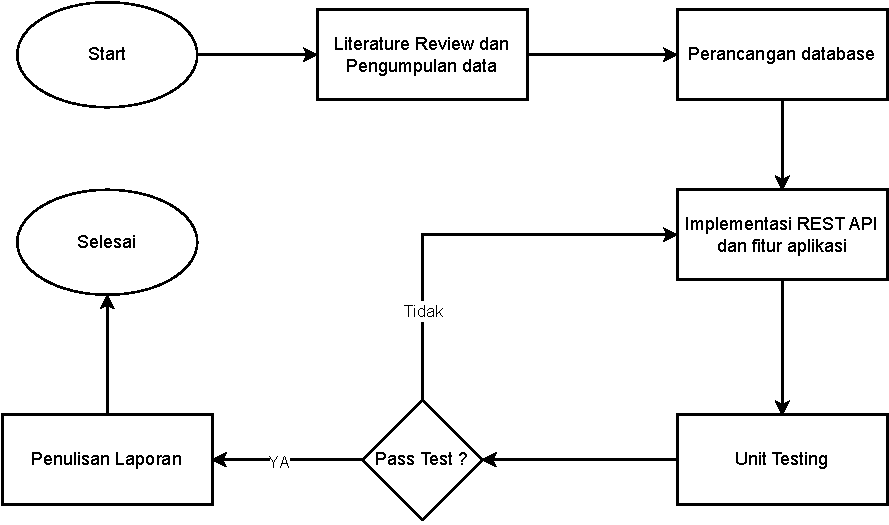
\includegraphics[width=0.75\textwidth]{drawio/alur-perancangan.drawio.pdf}
	\caption{Alur Perancangan}
	\label{alur-perancangan}
\end{figure}
Gambar \ref{alur-perancangan} menunjukkan alur perancangan sistem \textit{backend} yang dibuat. Terdapat 5 tahapan dalam perancangan sistem yaitu :

\subsection{\textit{Literature Review} dan Pengumpulan data}
Pada tahap ini, dilakukan pengumpulan data melalui Software Requirement Specification (SRS) yang telah dibuat oleh System Analyst (SA) serta membaca literatur ilmiah mengenai pengembangan \textit{backend} web.

\subsection{Perancangan database}
Pada tahap ini dilakukan perancangan dan implementasi ERD menggunakan PrismaJs sebagai \textit{framework} Object Relational Mapping.

\subsection{Implementasi REST API dan fitur aplikasi}
Pada tahap ini dilakukan sesi koding untuk mengimplementasikan berbagai macam fitur aplikasi berdasarkan SRS yang telah dibuat dan membuat API \textit{endpoint} yang menghindari \textit{anti pattern}.

\subsection{Unit Testing}
Pada tahap unit testing, dilakukan pengujian logic dan fungsi API, sampai tidak terdapat error lagi, maka dilanjut ke penulisan proposal.

\subsection{Penulisan laporan}
Pada tahap ini, akan disusun semua tahapan pekerjaan, hasil analisis dan pembahasan terhadap semua yang telah dilakukan, diamati, dan dihasilkan dalam membuat dan mengimplementasikan \textit{backend} aplikasi.

\section{Desain Sistem}
\begin{figure}[h]
	\centering
	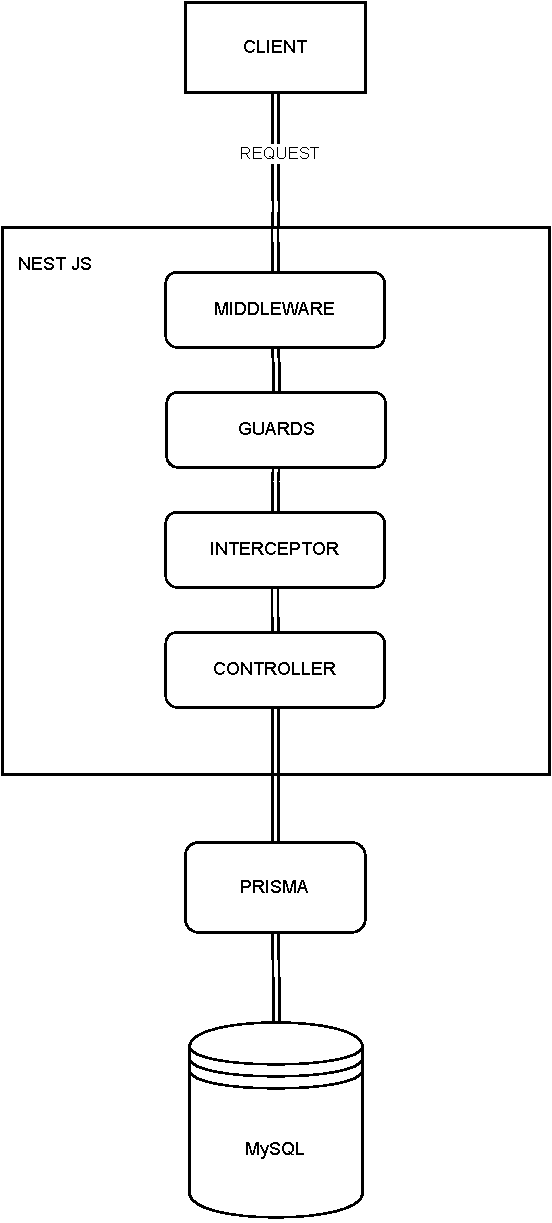
\includegraphics[width=0.35\textwidth]{drawio/sistem-desain.drawio.pdf}
	\caption{Desain Sistem}
	\label{sistem-desain}
\end{figure}
Implementasi dan perancangan RESTful API, Database, dan fungsi bisnis dikembangkan menggunakan \textit{framework} NestJs. Pada NestJs terdapat beberapa komponen seperti: Middleware, Guards, Interceptor, Controller, dan Service. Service yang dipakai adalah PrismaJs untuk menghubungkan NestJs ke \textit{Database System}. Gambar \ref{sistem-desain} merupakan \textit{Request Lifecycle} yang menjelaskan bagaimana alur \textit{request} ditangani dari awal sampai akhir.
Pada Middleware, fungsi akan dipanggil sebelum masuk ke routing. Pada Guard, \textit{request} akan dicek \textit{authenticity}, untuk mengetahui validitas dari \textit{request} tersebut. Tahap ini juga akan dicek keamanan session menggunakan JWT dan CSRF. Setelah melalui Guard, Request akan masuk ke Interceptor. Dimana jika suatu \textit{request} mempunyai suatu karakteristik yang ditentukan, maka akan menjalankan fungsi tambahan. Interceptor terjadi ketika \textit{request} datang \textit{(pre)}, dan response \textit{(post)}. Setelah melewati Interceptor, fungsi di Controller akan dijalankan. Jika pada Controller tersebut perlu data dari database maka akan turun ke service PrismaJs untuk melakukan database call menggunakan ORM \cite{NestJS}.

\begin{figure}[h]
	{\centering {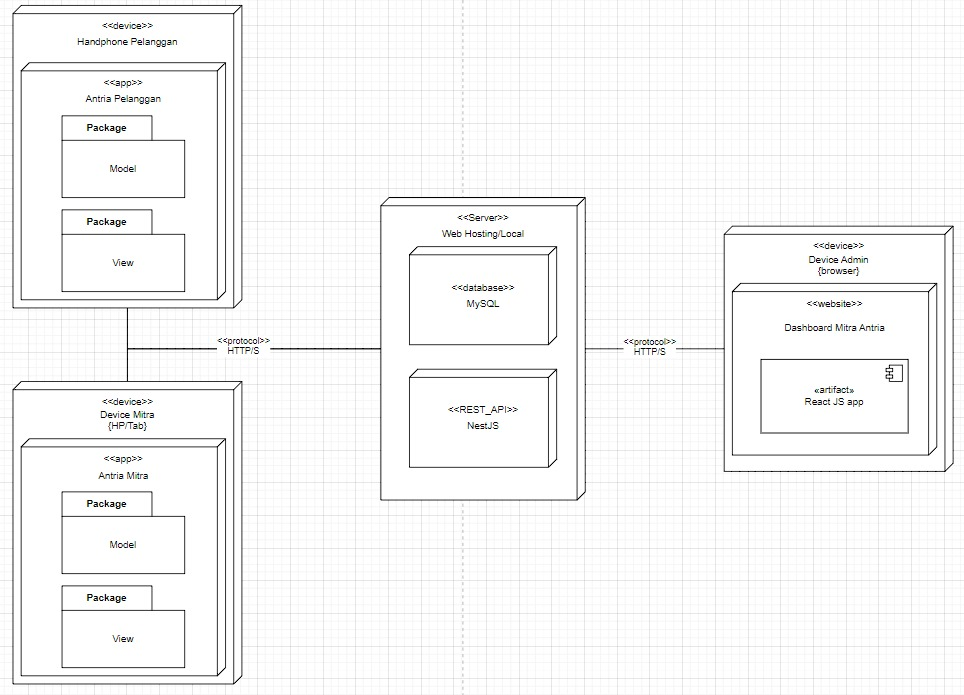
\includegraphics[scale=0.5]{drawio/deployment.jpg}}\par}
	\caption{Deployment Diagram}
	\label{deployment}
\end{figure}
Pada diagram \ref{deployment} menjelaskan bagaimana server backend berkomunikasi dengan Aplikasi lain melalui protokol HTTPS. 


%

%%%%%%%%%%%%%%%%%%%%%%%%%%%%%%%%%%%%%%%%%%%%%%%%%%%%%%%%%%%%%%%
% Berikut adalah untuk membuat Daftar pustaka
% Style daftar pustaka dapat disesuaikan dengan mengubah 
%\bibliographystyle{kode}
% dengan kode = acm maka hasinya contoh [1]
% dengan kode = agsm maka hasilnya Harvard style (Sukimin, 2017)
%%%%%%%%%%%%%%%%%%%%%%%%%%%%%%%%%%%%%%%%%%%%%%%%%%%%%%%%%%%%%%%%
\cleardoublepage
\addcontentsline{toc}{chapter}{Daftar Pustaka}

\bibliographystyle{acm} %harvard style
\bibliography{References}
%
%\pagebreak
%%%%%%%%%%%%%%%%%%%%%%%%%%%%%%%%%%%%%%%%%%%%%%%%%%%%%%%%%%%%%%%
% Berikut untuk lampiran
%%%%%%%%%%%%%%%%%%%%%%%%%%%%%%%%%%%%%%%%%%%%%%%%%%%%%%%%%%%%%%
\cleardoublepage
\addcontentsline{toc}{chapter}{Lampiran}
\chapter*{Lampiran}

\end{document}
